\section{Mathematical model}
Each of the two rotors of Ingenuity generates a thrust vector in a commanded direction, which is applied on the rotating hub. Not only does this result in a force capable of moving the helicopter, but it also generates a torque that can be used to control its orientation. \\The helicopter is treated as a simple rigid body without taking into account the aerodynamics of the blades, therefore the only external force is gravity. 

From now on, we will consider an inertial reference frame (superscript $^i$) and a non-inertial one attached to the drone body (superscript $^b$). \\ The relative orientation of the latter with respect to the former is expressed in roll, pitch and yaw angles (i.e. the three components of $W$), or alternatively through the corresponding rotation matrix (in compact trigonometric notation with $\sin(W_i) = s_i$ and $\cos(W_i) = c_i$):
\begin{align*}
    R(W) = R = \begin{bmatrix}
        c_2 c_1& s_2 s_1 c_3 - s_1 c_3 & s_3 s_2 c_1 + s_1 s_3 \\
        c_2 s_3 & s_2 s_1 s_3 + c_3 c_1 & s_3 s_2 c_1 - s_1 c_3 \\
        -s_2 & s_1 c_2 & c_2 c_1
    \end{bmatrix}
\end{align*}

\subsection{Helicopter dynamics}
The magnitude of the thrust generated by each of the rotors is given by the sum of two components, one due to the lift and the other due to the drag. 
\begin{gather*}
    F_l = K_l \omega^2, \\
    F_d = K_d \omega^2,
\end{gather*}
where $\omega$ represents the angular velocity of the rotor, while $K_l$ and $K_r$ are two coefficients, whose expressions are the following:
\begin{gather*}
    K_l = \frac{1}{2} C_l c r^3 \rho, \\
    K_d = \frac{1}{2} C_d c r^3 \rho.
\end{gather*}
In the previous formulas, $c$ is the chord of a rotor blade and $r$ is its hub-to-tip length; $\rho$ is the air density, while $C_l$ and $C_d$ indicate the lift and drag coefficients of the rotor blades, which depend on their angle of attack. We consider the latter constant at a value such that $K_l - K_d > 0$.\\
This means that we can write the total thrust norm generated by each rotor as:
\begin{gather}
    ||F|| = F_l - F_d = (K_l - K_d) \, \omega^2, \label{eq:force_norm}
\end{gather}
therefore we can treat $\omega_u$ and $\omega_l$ as two of the control inputs of the system (respectively, for the upper and lower rotor).

Now consider the angles that the projections of the thrust vectors on the planes $xz$ and $yz$ form with the vertical axis $z$, called respectively $\alpha$ and $\beta$: this couple is the other input of the system, and it is the same for the upper and lower rotors. The two angles are illustrated in Figure \ref{fig:alpha_beta}.

\begin{figure}[H]
    \centering
    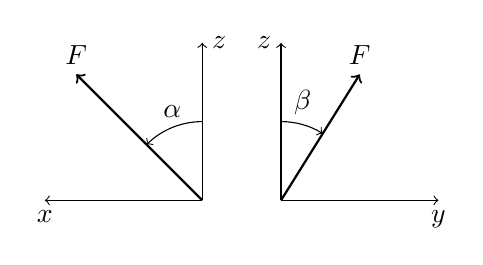
\begin{tikzpicture}[scale=2]
        \draw[->] (0,0) -- (0,1) node[right] {$z$};
        \draw[->] (0,0) -- (-1,0) node[below] {$x$};
        
        \draw[->,thick] (0,0) -- (-0.8,0.8) node[above] {$F$};
        
        \draw[->] (0,0.5) arc (90:135:0.5) node[midway, above] {$\alpha$};

        \draw[->] (0.5,0) -- (0.5,1) node[left] {$z$};
        \draw[->] (0.5,0) -- (1.5,0) node[below] {$y$};
        
        \draw[->,thick] (0.5,0) -- (1,0.8) node[above] {$F$};
        
        \draw[->] (0.5,0.5) arc (90:58:0.5) node[midway, above] {$\beta$};
    \end{tikzpicture}
    \caption{Angles $\alpha$ and $\beta$ that the projections of the thrust vector forms with the vertical direction in the $xz$ and $yz$ planes of the body frame.}
    \label{fig:alpha_beta}
\end{figure}

\noindent In the body reference frame, the thrust vector is then written by means of the auxiliary angle $\gamma$, i.e. the angle that the thrust vector forms with the vertical axis $z$ in the three-dimensional space:
\begin{align}
    F^b = T_{(\alpha, \beta)}||F|| \label{eq:force}
\end{align}
\vspace*{-0.6cm}
\begin{align*}\text{with} \quad T_{(\alpha, \beta)} = \begin{bmatrix}
        -\tan{\alpha} \cos{\gamma} \\
        -\tan{\beta} \cos{\gamma} \\
        \cos{\gamma}
    \end{bmatrix}, \\
    \tan^2{\gamma} = \tan^2{\alpha} + \tan^2{\beta}. 
\end{align*}

Since the thrust vectors are not applied in the center of mass of the helicopter, they also generate torques according to:
\begin{align} 
    \tau^b = \begin{bmatrix}
        0 \\ 0 \\ d_{cm}
    \end{bmatrix} \times F^b, \label{eq:torque_due_force}
\end{align}
with $d_{cm}$ being the distance between the center of mass of the helicopter and the center of the rotors.\\
Note that this cross product results in a vector whose last component is null. In fact, the yaw rotation is caused by the difference of the reaction torques generated by the two rotors:
\begin{align} 
    \tau^b_r = \begin{bmatrix}
        0 \\ 0 \\ Q_u - Q_l
    \end{bmatrix} \quad \text{with} \quad Q = 0.02 \; ||F||. \label{eq:reaction_torque}
\end{align}

According to Newton's second law, the overall force acting on the helicopter is the sum of the forces generated by the two rotors and the force of gravity:
\begin{gather*}
    \begin{split}
        F^b_{tot} & = F^b_u + F^b_l + R^T F^i_g \\
        & = T_{(\alpha, \beta)} (K_l - K_d) (\omega^2_u + \omega^2_l)+ R^T F^i_g,
    \end{split}
\end{gather*}
where \(F^b_{tot}\) is the total force acting on the body and \(F^i_{g}\) is the gravitational force.
Similarly, the total torque is composed of the torques generated by the two rotor thrust vectors (roll and pitch) and the reaction torque of the two rotors (yaw):
\begin{align}
    \tau^b_{tot} = \tau^b_u + \tau^b_l + \tau^b_r,
    \label{eq:torque}
\end{align}
where $\tau_{tot}^b$ is the total torque acting on the body.

By applying these laws, we compute the derivative of the velocity $V$ in the body frame. Neglecting external forces, the cross product term accounts for the Coriolis effect.
This is also done for the angular velocity $\Omega$, where the cross product term represents the gyroscopic effect.
\begin{gather*}
    \frac{d}{dt}{V^b} = \frac{F^b_{tot} - \Omega^b \times (m V^b)}{m}, \\
    \frac{d}{dt}{\Omega^b} = I^{-1} (\tau^b_{tot} - \Omega^b \times (I \Omega^b)).
\end{gather*}
In the inertial frame, the position $P$ and the orientation $W$ of the robot are updated by integrating the velocity and the angular velocity, with:
\begin{gather*}
    \frac{d}{dt}P = R\, V^b, \\ 
    \frac{d}{dt}W = R\, \Omega^b.
\end{gather*}
\subsection{Actuator dynamics}
The control signals $\omega_u$, $\omega_l$, $\alpha$ and $\beta$ are not instantly translated into the corresponding angular velocities or swashplate tilt angles: non-idealities arise since the physical components of Ingenuity are set in motion by actuators (typically electrical motors). \\
In reality, often actuators integrate low-level closed loops (sometimes even analog, e.g. through potentiometers) whose dynamics may be overlooked in the high-level control system design.
To account for the effect of these components in our model and simulations, however, it is appropriate to model each of the four input channels as double integrators:
\begin{align*}
    G_i(s) = \frac{1}{s^2}, \quad i = 1, 2, 3, 4.
\end{align*}
In feedforward, the trivial solution is to control the double integrators with (physically realizable) controllers such as:
\begin{align*}
    K_i(s) = \frac{s^2}{(1 + s \, T_i)^2}, \quad i = 1, 2, 3, 4,
\end{align*}
with $T_i$ being a (small enough) time constant that can be tuned to match the actual dynamics of the actuators. \\
This means that, at the end of the day, the resulting actuator open-loop transfer functions are equal to:
\begin{align*}
    L_i(s) = G_i(s) \, K_i(s) = \frac{1}{(1 + s \, T_i)^2}, \quad i = 1, 2, 3, 4.
\end{align*}